\chapter{پژوهش‌های پیشین}\label{Chap:Chap2}
\minitoc

\section{مقدمه}\label{intro}

\subsection{پیش‌نیازها}
مدل‌های زبانی ارائه شده را می‌توان به دو دسته کلی تقسیم نمود. روش‌های \trans{نمادین}{Symbolic} و روش‌های آماری. روش‌های نمادین، روش‌هایی قدیمی‌تر بوده و بیشتر بر اساس قوانین از پیش تعریف شده کار می‌کنند. این قوانین دقت بالایی در رعایت قوانین دستور زبان دارند اما \trans{فراخوانی}{Recall} پایینی دارند؛ چرا که این قوانین تمامی پیچیدگی‌های زبان را مدل نمی‌کنند.\\
در مقابل روش‌های آماری قرار دارند که پایه آن‌ها مبنی بر پیش‌بینی کلمه بعدی با داشتن کلمه‌های پیشین است. در این رویکرد، هر کلمه یک متغیر تصادفی بوده که مقدار آن نمایانگر کلمه جاری و تابعی از کلمات پیشین است. این گونه از دنباله متغیر‌های تصادفی را مدل‌های \trans{خودبرگشتی}{Auto-regressive} می‌نامند. اگر $X_t$ متغیر تصادفی متناظر با کلمه $t$ام و طول جمله $T$ باشد، طبق قانون زنجیره‌ای خواهیم داشت:
\begin{equation}\begin{split}
		p(X_1, X_2, ... , X_T) = p(X_1) p(X_2|X_1) p(X_3|X_2, X_1) ... p(X_T|X_1, ..., X_{T-1}).
	\end{split}\end{equation}
که در واقع به دنبال مدل کردن $p(X_t|X_1, ..., X_{t-1 })$ هستیم. \\
قرارداد می‌کنیم توزیع $P$ مربوط به توزیع داده واقعی باشد و در مقابل آن به دنبال یافتن توزیع $Q$ هستیم که تا حد ممکن نزدیک به $P$ باشد.
از آنجا که در طول متن گزارش، فاصله‌های گوناگونی مورد استفاده قرار گرفته است، در ابتدا آن‌ها تعریف می‌کنیم. در تمامی تعاریف، P مربوط به توزیع اصلی و Q مربوط به توزیعی است که یاد گرفته می‌شود.

\subsubsection{فاصله  \lr{KL}}
فاصله ‎\lr{KL} به شکل زیر تعریف می‌شود.
\begin{gather} \label{eq: kl}
	KL (P || Q)   = \sum_x p(x) \log \frac{p(x)}{q(x)}
\end{gather}
تحلیل رفتاری:
همان طور که در رابطه ‎\ref{eq: kl}‎ مشخص است،
‎\subsubsection{فاصله \lr{KL} معکوس}
\subsubsection{فاصله \lr{Jensen Shannon}}
این فاصله که فاصله JS نیز نامیده می‌شود.
\subsubsection{فاصله \lr{Total Variation}}
\subsubsection{فاصله \lr{Wasserstein}}
\section{مدل زبانی با فضای نهان یا بدون فضای نهان؟}
پیش از آنکه در مورد مدل‌های زبانی ارائه شده صحبت شود، لازم است تا در ابتدا این مدل‌ها را به دو دسته تقسیم کنیم. مدل‌های با فضای نهان و بدون فضای نهان. مدل‌های زبانی با فضای نهان به این صورت هستند که فرض شده است جملات در فضای نهان ‎کد شده و شبکه ‎\decoder یی با دریافت برداری از فضای نهان، آن را به جمله مربوطه برگردان می‌کند. با داشتن چنین قابلیتی امکان کنترل کردن شبکه ‎\decoder{}‎ وجود داشته و حتی می‌توان با حرکت روی این فضا جملات شبیه به یکدیگر تولید نموده و یا از یک جمله شروع کرده و به مرور با تغییر بردار ورودی (از فضای نهان) آن به جمله دیگری تبدیل کنیم. این در حالیست که مدل‌های زبانی بدون فضای نهان از این قابلیت بی‌بهره بوده و نمی‌توان کنترلی بر نحوه خروجی آن‌ها داشت.
\section{مدل‌های زبانی بدون فضای نهان}
\subsection{مدل زبانی پایه (\teacherforcing{})}
مدل \trans{جبر معلم}{Teacher forcing} شاید ساده‌ترین دسته از مدل‌های تولید متن با استفاده از شبکه‌های عصبی باشد. آموزش این مدل‌ها مبتنی بر بیشینه کردن \trans{درست‌نمایی}{Likelihood} داده آموزش در مدل است \cite{teacher-force}. اگر پارامترهای مدل را با $‎\theta$ نشان دهیم، تابع هزینه این مدل به صورت زیر است:
\begin{equation}\begin{split}
		L_{MLE} = -\expected_{x \sim P_{data}(x)} [\log p_\theta (x)] = -\expected_{x \sim p_{data}(x)} [\log p_\theta (x_1) + \sum_{t=2}^{T}  +\log p_\theta (x_t|x_1, ..., x_{t-1})].
	\end{split}\end{equation}

\begin{figure}[H]
	\centering
	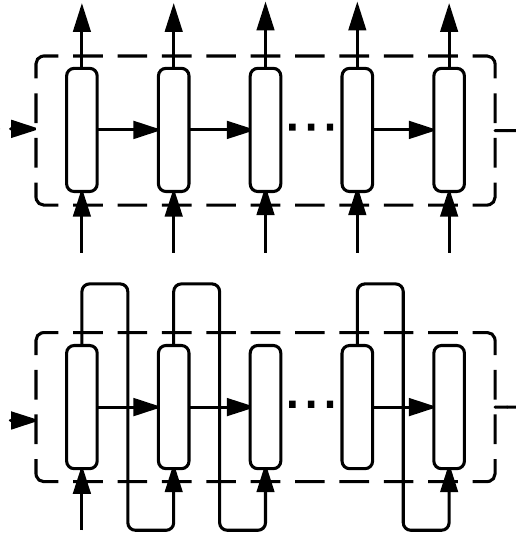
\includegraphics[width=0.25\textwidth]{images/teach-prof.png}
	\caption{
		تفاوت بین آموزش و آزمون مد‌ل جبر معلم. شکل بالا مربوط به زمان آموزش و شکل پایین مربوط به زمان آزمون است. \cite{prof-force}.}
	\label{fig:expbias}
\end{figure}

به عبارت دیگر، در هر زمان درست‌نمایی هر کلمه را با داشتن کلمات قبلی بیشینه می‌کنیم. \\
همان‌طور که از روابط تابع هزینه مشخص است، آموزش این دسته از مدل‌ها ساده بوده اما دچار پدیده‌ای به نام \trans{اریبی مواجهه}{Exposure bias} هستند \cite{ prof-force, ssampling}. این مشکل ناشی از تفاوت رفتار با مدل حین آموزش و حین آزمون است. همان طور که در شکل \ref{fig:expbias} مشخص است، حین آموزش، در هر زمان، کلمات کاملا درست تحویل مدل شده، در حالی که در زمان آزمون ورودی شبکه در هر زمان، با استفاده از نمونه‌گیری از خود مدل در زمان قبل ساخته می‌شود. از آنجا که مدل مفهوم کاملا درستی را نیاموخته است، کلمه‌ی تولید شده برای ورود به زمان بعد، کلمه کاملا صحیحی نبوده و چنین رفتاری باعث می‌شود تا مدل، ورودی‌ای را دریافت کند که دارای مقداری خطا بوده که در زمان آموزش مانند آن را ندیده است (کلمات کاملا صحیح ورودی شبکه بوده‌اند)؛ این رفتار در طول تولید هر کلمه از یک جمله با هم تجمیع شده و در نهایت منجر به تولید جمله‌ای نه چندان صحیح خواهد شد.\\
به منظور رفع این مشکل، روش‌های متفاوتی ارائه شد \cite{prof-force, ssampling} که در بخش \ref{sec:gan} به عنوان یکی از راه‌حل‌ها به آن پرداخته خواهد شد.
از دیگر مشکلات این روش باید به تفاوت تابع هزینه و معیار ارزیابی اشاره کرد؛ به عبارت دیگر اگر معیار ارزیابی، معیاری مانند \lr{BLEU} باشد، هدف ارزیابی کسب امتیاز بالاتر \lr{BLEU} است و نه افزایش درست‌نمایی داده آموزش و لزوما افزایش درست‌نمایی به افزایش ‌\lr{BLEU} منجر نمی‌شود.
\subsection{مدل زبانی با استفاده از \gan{}}
شاید \trans{‎\gan}{Generative adversarial networks} یکی از مطرح‌ترین و موفق‌ترین مدل‌های مولد حال حاضر می‌باشند. این شبکه‌ها که مجددا ابتدا در حوزه تصویر معرفی شدند، از دو بخش کلی تشکیل شده اند \cite{gan}؛ بخش \trans{مولد}{Generator} و بخش \trans{تمیزدهنده}{discriminator}. همان‌طور که از نام‌گذاری آن‌ها مشخص است، مولد وظیفه تولید نمونه‌های مصنوعی و تمیزدهنده وظیفه تشخیص نمونه مصنوعی از واقعی را دارد. نحوه آموزش آن‌ها به این صورت است که مولد سعی در تولید نمونه‌های شبیه به داده واقعی داشته و تمیزدهنده در جهت مخالف سعی در شناسایی این نمونه‌ها دارد. در واقع نوعی \trans{بازی کمینه-بیشینه}{Min-max game} بین مولد و تمیزدهنده در جریان است. تابع هدف این مدل به شرح زیر است:
\begin{equation} \label{eq:gan}
	\begin{split}
		V_{GAN} (G, D) = \expected_{x \sim p_{data}(x)} [\log D(x)] + \expected_{z \sim p(z)} [\log (1 - D(G(z)))]
	\end{split}
\end{equation}
که  $p(z)$ توزیع پیشین تعریف شده بر روی نویز $z$،
$G(z)$
تابع مولد (تبدیل کننده نویز $z$ به نمونه $x$)، $D(x)$ تابع تمیزدهنده بوده و این رابطه برحسب $G$ کمینه و $D$ بیشینه می‌گردد.\\
اگر $q_G(x)$ نشان دهنده توزیع حاصل از اعمال تابع $G(z)$ به توزیع پیشین $p(z)$ باشد؛ نشان داده شده است که نقطه بیشینه کننده رابطه \ref{eq:gan} بر حسب $D$، به صورت زیر است:
\begin{gather}
	D_G^*(x) = \frac{p_{data}(x)}{p_{data}(x) + q_G(x)}
\end{gather}
با فرض رسیدن به تمیزدهنده بهینه، کمینه کردن $V(D^*_G,G)$ معادل کمینه کردن فاصله \lr{Jensen Shannon} بین $p_{data}(x)$ و $q_G(x)$ خواهد بود.

به مانند شبکه‌های \vae{}، \gan{} نیز حداقل در ابتدا در حوزه متن چندان موفق نبوده و به دلیل مشکلی که به آن اشاره خواهد شد، مدتی از حوزه تصویر عقب ماند. این مشکل از نحوه آموزش نشأت می‌گیرد. همان طور که در روابط تابع هزینه مشخص است، تمیزدهنده باید به نمونه‌های تولید شده توسط مولد عددی نزدیک به صفر نسبت دهد. آنچه که باید در آموزش و الگوریتم \trans{گرادیان کاهشی تصادفی}{Stochastic gradient descent} محاسبه شود، محاسبه مشتق تابع هزینه نسبت به پارامتر‌های شبکه مولد است؛ اما از آنجا که شبکه مولد مستقیما در تابع هزینه شرکت نکرده و نمونه‌های تولیدی آن شرکت می‌کنند و عملیات نمونه‌گیری در فضای گسسته عملیاتی مشتق‌ناپذیر است، بنابراین امکان گذر گرادیان از تابع هزینه (شبکه تمیزدهنده) به شبکه مولد به سادگی وجود ندارد. در واقع شبیه چنین مشکلی در شبکه‌های \vae{} نیز وجود دارد اما با تکنیکی به نام \trans{پارامتریزه‌سازی مجدد}{Reparameterization} که منبع تزریق عامل تصادفی (نمونه‌گیری) را از مسیر انتقال گرادیان خارج می‌کند، حل شده است.\\
به منظور حل این مشکل نیز رویکرد‌های متفاوتی ارائه شده است که به یکی و شاید معروف‌ترین از آن‌ها اشاره خواهد شد.\\
\subsubsection*{\lr{SeqGAN}}
در روش \lr{SeqGAN} راه حل ارائه شده برای مشکل گذر گرادیان الهام گرفته شده از حوزه \trans{یادگیری تقویتی}{Reinforcement Learning} است \cite{seqgan}؛ در واقع همین مشکل به نوعی دیگر در حوزه یادگیری تقویتی مطرح است و با روشی به نام روش \trans{گرادیان سیاست}{Policy gradient} رفع شده است. ساختار یک مسئله حوزه یادگیری تقویتی شامل ۴ بخش است که با تعریف تمام بخش‌های آن، ‌می‌توان بخش آموزش مولد در \gan{} را به عنوان آموزش یک عامل با روش \reinforce{} دید. این بخش‌ها شامل موارد روبرو هستند: فضای حالت عامل ($S$)، فضای عمل عامل ($A$)، \trans{تابع گذار}{Transition function}
(\lr{$T(s,a)$})
و \trans{تابع پاداش}{Reward function}
(\lr{$R(s,a)$}).
\begin{equation}\begin{split}
		\nonumber
		T: S \times A \rightarrow S\\
		R: S \times A \rightarrow \mathbb{R}
	\end{split}\end{equation}
در اینجا حالت فعلی عامل، \trans{بازنمایی}{Representation} کلمات تولید شده تا به حال، عمل عامل،‌کلمه انتخابی بعدی، حالت بعدی، تجمیع کلمات قبلی تولید شده و کلمه فعلی و تابع پاداش، امتیاز میزان واقعی بودن جمله‌ای است که تمایز دهنده به جمله تولیدی نسبت می‌دهد، است. بدیهی است که تابع گذار تابعی \trans{قطعی}{Deterministic} بوده و پاداش مورد نظر بعد از تولید کامل جمله به عامل داده می‌شود. در این حالت رابطه گرادیان تابع مولد به شکل زیر بدست خواهد آمد.
\begin{equation} \label{eq:seqgan-grad}
	\begin{split}
		\nabla_G L_{GAN} (G, D) &= \nabla_G \expected_{x \sim G(x)} [\log D(x)]= \expected_{x \sim G(x)} [\log D(x) \nabla_G \log G(x)].
	\end{split}
\end{equation}

\begin{figure}[t]
	\centering
	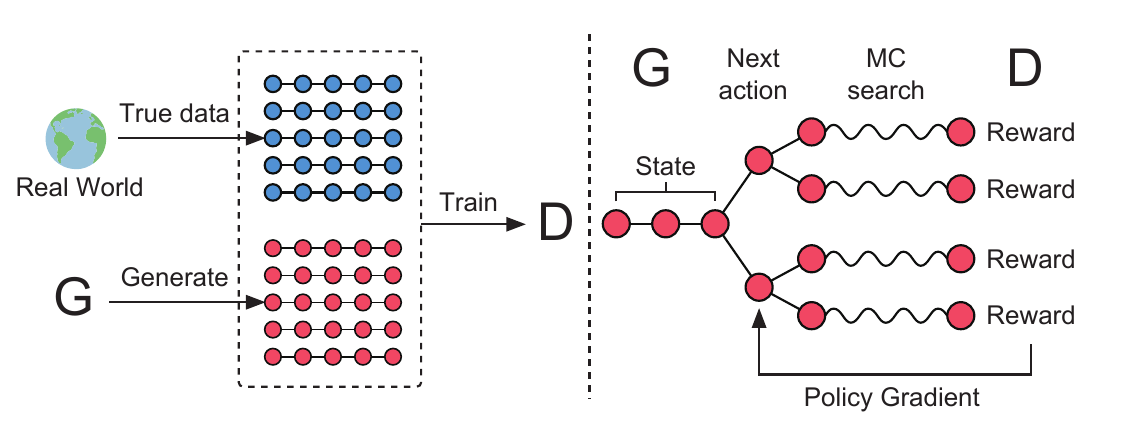
\includegraphics[width=0.5\textwidth]{images/seq-gan.png}
	\caption{
		نمایی نحوه آموزش مدل \lr{SeqGAN}
		\cite{seqgan}.}
	\label{fig:seq-gan}
\end{figure}

همان‌طور که در شکل \ref{fig:seq-gan} و رابطه \ref{eq:seqgan-grad} مشخص است، عامل طبق سیاستی که تا به حال بدست آورده است، تعدادی نمونه ایجاد نموده و به نسبت پاداش دریافتی به ازای هر نمونه، درست‌نمایی نمونه‌های مرتبط را افزایش خواهد داد.\\
نکته قابل توجهی که لازم است تا به آن اشاره شود، توانایی این روش در حل مشکل \expbias{} است. در واقع از یک سو در هر زمان کلمه بعدی توسط خود مدل تولید می‌شود و از سوی دیگر پاداشی که از تمیزدهنده دریافت می‌کند، میزان میزان واقعی بودن کل جمله است؛ بنابراین اگر جمله تولید شده از نظر تمیزدهنده، کیفیت لازم را نداشته باشد، تمیزدهنده امتیاز کمتری به آن نسبت خواهد داد و گرادیان متناسب به مولد اعمال خواهد شد. با اینکه این روش مشکل ذکر شده را حل می‌کند اما فضایی که عامل باید در آن به دنبال یافتن پاداش بیشینه باشد نمایی بوده و همین امر آموزش این دسته از مدل‌ها را با چالش روبرو می‌کند. پیشنهاد ساده‌ای که برای این موضوع ارائه می‌شود استفاده از پیش آموزش به روش \teacherforcing{} است. در واقع ابتدا مدل به یک \trans{بهینه محلی}{Local optimum} رسیده و در فضای نزدیک به آن احتمالا پاداش بیشتری نسبت به حالتی که مدل تصادفی باشد دریافت کرده و به اصلاح خود می‌پردازد.\\
این روش تنها مدل موجود با چنین رویکردی نبوده و روش‌هایی همچون \cite{pgbleu} از دانش خبره مانند معیار \lr{BLEU} به عنوان پاداش بهره برده‌اند.
\section{مدل‌های زبانی با فضای نهان}
\subsection{\vae{}}
اولین دسته، مدل \trans{خودرمزنگار وردشی}{Variational autoencoder} است \cite{vae-org}. با معرفی این دسته از مدل‌ها، موج جدیدی در حوزه مدل‌های مولد به طور خاص مدل‌های مولد تصویر ایجاد شد.
\begin{figure}[H]
	\centering
	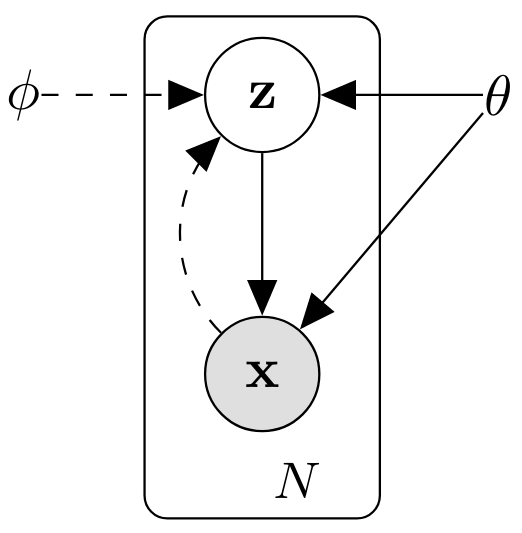
\includegraphics[width=0.25\textwidth]{images/vae-pgm.png}
	\caption{
		نمایی از مدل گرافی مورد استفاده در \vae{}. خطوط خطچین‌‌دار مربوط به تخمین توزیع پسین $p_\theta(z|x)$ و خطوط بدون خطچین مربوط به مدل مولد $p_\theta(x|z)$ است.
		\cite{vae-text}.}
	\label{fig:vae-pgm}
\end{figure}
این ساختار به منظور یادگیری و \trans{\inference}{Inference} مدل‌های با مدل گرافی نشان داده شده در شکل ‎\ref{fig:vae-pgm}‎ ارائه شده است. در واقع در این مدل، هر داده از یک \trans{\latentvar}{Latent Variable}  تولید شده که \priordist{} مشخصی برای آن تعریف شده است و معمولا توزیع گاوسی نرمال است. از آنجا که محاسبه $\log p_\theta(x)$ ن و $\log p_\theta (z|x)$ نیازمند \inference ی \trans{سخت}{Intractable} است، با بهره‌گیری از  توزیع وردشی $q_\phi(z|x)$، کران پایینی از \likelihood{} را بیشینه می‌گردد.\\
از دیدگاهی دیگر، این مدل از دو بخش کلی تشکیل شده است؛ \trans{کدگذار}{encoder} و \trans{کدگشا}{decoder}. بخش \encoder{} وظیفه کد کردن داده ورودی در فضای نهان را داشته و در مقابل \decoder{} وظیفه برگرداندن فضای نهان به داده اصلی. تفاوت این مدل‌ها با \trans{خودرمزنگار}{autoencoder}ها در فرض و اعمال توزیع نرمال بر فضای نهان است؛ به همین دلیل امکان نمونه‌برداری از فضای نهان امکان‌پذیر خواهد بود. تابع هزینه در این ساختار، به شکل زیر تعریف شده است:
\begin{equation} \label{eq:vae}
	\begin{split}
		L_{VAE} = \expected_{x \sim p_{data}(x)} [KL(q_\phi(z|x) || N(\textbf{\latin{0}},\textbf{\latin{I}}))- \expected_{z \sim q_\phi(z|x)}[\log p_\theta(x|z)]]
	\end{split}
\end{equation}


که $q_\phi(z|x)$ تابع توزیع \encoder{} و $p_\theta(x|z)$ تابع توزیع \decoder ست. همان طور که مشخص است، تابع هزینه از دو بخش کلی تشکیل شده است. قسمت اول وظیفه اجبار کردن تابع توزیع \encoder{} به کد کردن داده‌ها در فضای گاوسی نرمال و بخش دوم نیز وظیفه کمینه کردن خطای بازسازی داده ورودی را بر عهده دارد. بنابراین شبکه سعی در یادگرفتن مدلی دارد که علاوه بر داشتن خطای بازسازی کم، توزیع گاوسی نرمال نیز بر فضای نهان آن حاکم باشد؛ پس می‌توان بعد از آموزش مدل، با نمونه‌گیری از توزیع نرمال و کدگشایی آن توسط $p_\theta(x|z)$ داده مصنوعی تولید نمود. از آنجا که معمولا از توزیع گاوسی نرمال به عنوان \priordist{} استفاده میگردد و خروجی \encoder{} نیز توزیعی گاوسی با ماتریس کوارایانس قطری است، عبارت $KL(q_\phi(z|x) || N(\textbf{\latin{0}},\textbf{\latin{I}}))$ به صورت فرم بسته قابل محاسبه خواهد بود. نکته قابل توجه این است که طبق رابطه \ref{eq:vae}، سعی بر این است تا خروجی \encoder{} به ازای هر نقطه، مستقلا، به توزیع گاوسی نرمال نزدیک باشد؛ بنابراین این قسمت از تابع هزینه، محدودیت زیادی را بر روی خروجی \encoder{} اعمال کرده و همان طور که در آینده توضیح داده خواهد شد، فرآیند آموزش آن را در بعضی حوزه‌ها دچار مشکل می‌کند. \\
\subsubsection{تکنیک \reparametrization{}}
\subsubsection{تکنیک \reparametrization{}}

\begin{figure}[H]
	\centering
	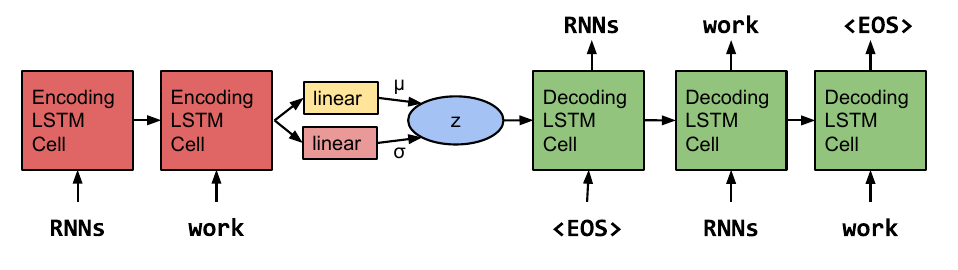
\includegraphics[width=0.5\textwidth]{images/vae-text.png}
	\caption{
		نمایی از مدل \vae{} استفاده شده در حوزه متن
		\cite{vae-text}.}
	\label{fig:vae-text}
\end{figure}
آنچه که در حوزه متن اتفاق می‌افتد، صفر شدن قسمت شامل فاصله \lr{KL}  است؛ در واقع می‌توان این طور بیان کرد که کدگذار بدون توجه به معنی‌دار بودن فضای نهان، هر جمله را مستقلا به یک نقطه از فضای نهان نگاشت می‌کند. در نتیجه‌ی این روند، کدگشا هم مستقل از معنای فضای نهان جمله‌ای را تولید خواهد نمود و توزیع نرمال فرض شده بر فضای نهان یک جمله، چندان حاوی جملات مشابه آن نخواهد بود و روند آموزش به مشکل بر خواهد خورد. \\
به منظور دور زدن این مشکل از اعمال تغییراتی در معماری شبکه، تابع هزینه و روند آموزش بهره برده می‌شود \cite{improved-text-vae, hybrid-text-vae} اما همچنان این معضل به طور کامل رفع نمی‌شود. یکی از مهم‌ترین تغییرات، دخیل کردن تدریجی قسمت حاوی \lr{KL} به تابع هزینه است. تابع هزینه به صورت زیر تغییر می‌کند:
\begin{equation}
	\begin{split}
		L_{VAE} = \expected_{x \sim p_{data}(x)} [\lambda_{KL} KL(q(z|x) || N(\textbf{\latin{0}},\textbf{\latin{I}}))- \expected_{z \sim q(z|x)}[\log p(x|z)]]
	\end{split}
\end{equation}
که $\lambda_{KL}$ ضریبی مثبت است. در واقع در ابتدا با قرار دادن $\lambda_{KL}=0$، مدل تنها یک خودرمزنگار ساده بوده و فضای نهان معنا داری ساخته و به مرور با میل دادن آن به یک، سعی در جمع کردن فضای نهان در فضای گاوسی نرمال خواهد داشت. جالب توجه است که چنین اتفاقی در حوزه تصویر رخ نمی‌دهد و قسمت \lr{KL} صفر نمی‌شود. این پدیده را شاید بتوان این طور توجیه کرد که از یک سو تغییرات ابتدایی فضای نهان زیاد بوده و دخیل کردن این تغییرات در تولید نمونه مورد نظر امری دشوار است؛ از سویی دیگر کدگشا به لحاظ معماری توانایی نگاشت هر نقطه از فضا را به جمله مورد نظر دارد و بنابراین رابطه تولید و استفاده از معنای فضای نهان بین کدگشا و کدگذار چندان شکل نمی‌گیرد.\\
گذشته از مشکلات ذکر شده، همان‌طور که در تابع هزینه آن دیده می‌شود همچنان کدگشا سعی در بالابردن درست‌نمایی داده آموزش را داشته و بنابراین این مدل همچنان مشکل \expbias{} را داشته و راه حلی برای این موضوع ارائه نمی‌کند.

به منظور رفع مشکل ذکر شده، کارهای متعددی از جهات مختلف آن را مورد بررسی قرار داده و راه حل‌هایی ارائه داده‌اند. در ادامه تعدادی از آن‌ها توضیح داده خواهند شد.
\subsection{عوامل صفر شدن \lr{KL}}
بررسی‌های مختلفی جهت شناسایی عوامل رخداد چنین پدیده‌ای صورت گرفته است که در ادامه به توضیح تعدادی از آن‌ها پرداخته خواهد شد.
\subsubsection{تمایل شبکه \decoder{}
	به استقلال داشتن از فضای نهان}
مقالات متعددی وجود دارند که به تحلیل \vae{} از دیدگاه نظریه اطلاعات پرداخته‌اند. یکی از این دیدگاه‌ها ارتباط روش کدینگ \bitsback{} با \vae{} است.\\
فرض کنید بخواهیم اطلاعات را با استفاده از فضای نهان \vae{} کد کنیم. از آنجا که تمام اطلاعات در فضای نهان کد نشده است باید خطای بازسازی را نیز کد کنیم. بنابراین هر کد از دو بخش
$\prob(z)$
(\priordist{})
و $\prob(x|z)$
(توزیع \decoder{})
تشکیل خواهد و میانگین طول کد به شرح زیر است:
\begin{gather}
	\mathcal{L}_{naive} = \expected_{x \sim \text{data}, z \sim q(z|x)} [-\log p(z) - \log p(x|z)]
\end{gather}
می‌توان روش کدینگ فوق را با استفاده از اطلاعات $q(z|x)$ بهبود داد؛ چراکه این توزیع به طور میانگین حداکثر $H(q(z|x))$  \lr{nats} اطلاعات در خود دارد. روش به این صورت خواهد بود که \decoder{} هنگام بازگشایی کد، به توزیع تخمینی $\prob(z|x)$ که فرستنده از آن استفاده می‌کند، دسترسی داشته و در نتیجه به اندازه $\log q(z|x)$ از طول کد کم خواهد شد. میانگین طول کد به صورت زیر تغییر خواهد کرد.
\begin{gather}
	\mathcal{L}_{\text{BitsBack}} = \expected_{x \sim \text{data}, z \sim q(z|x)} [\log q(z|x) -\log p(z) - \log p(x|z)]
\end{gather}
که برابر است با تابع هزینه \vae{}:
\begin{gather}
	\begin{align}
		\mathcal{L}_{\text{BitsBack}} = & \expected_{x \sim \text{data}} \Big[\expected_{z \sim q(z|x)} [\log p(x|z)] + KL\big(q(z|x) ~||~ p(z)\big)\Big] \nonumber
		\\
		=                               & \mathcal{L}_{\text{VAE}}
	\end{align}
\end{gather}
از سوی دیگر می‌توان کران پایینی برای تابع هزینه فوق بدست آورد که تابعی از آنتروپی توزیع داده اصلیست. می‌دانیم کران پایین میانگین طول کد برای کد کردن یک نوع داده، آنتروپی آن است. طبق روابط چنین بدست می‌آید:
\begin{align}
	\mathcal{L}_{\text{BitsBack}} =                                            & \expected_{x \sim \text{data}, z \sim q(z|x)} [\log q(z|x) -\log p(z) - \log p(x|z)] \nonumber
	\\
	=                                                                          & \expected_{x \sim \text{data}} [-\log p(x) + KL\big(q(z|x) ~||~ p(z|x)\big)] \nonumber
	\\
	\xrightarrow[\text{\lr{by Shannon entropy}}]{\text{\lr{lower bound}}} \geq & \expected_{x \sim \text{data}} [-\log p_{\text{data}}(x) + KL\big(q(z|x) ~||~ p(z|x)\big)] \nonumber
	\\
	=                                                                          & \mathcal{H}(\text{data}) + \expected_{x \sim \text{data}} [KL\big(q(z|x) ~||~ p(z|x)\big)]
\end{align}
بنابراین این روش کدینگ به اندازه
$KL\big(q(z|x) ~||~ p(z|x)\big)$
از کدینگ بهینه فاصله دارد و هر قدر این فاصله کمینه گردد، کدینگ نیز طبیعتا بهینه‌تر خواهد بود. \\
اما رابطه فوق چه کمکی به تحلیل پدیده صفر شدن \lr{KL} می‌کند. فرض کنید که \decoder{}
($p(x|z)$)
تابعی با قدرت مدل‌سازی بینهایت بوده و توانایی مدل کردن $p_{\text{data}}(x)$ را مستقل از $z$ دارد. از سوی دیگر این امکان برای $q(z|x)$ وجود دارد تا بر خلاف خواسته ما، ضمن عدم استفاده مفید از $x$ توزیعی صرفا برابر با $p(z)$ بسازد. در نتیجه می‌توان با این گونه مدلسازی با آنکه نه $q$ اطلاعات مفیدی را کد کرده و نه $p(x|z)$ از فضای نهان به درستی استفاده می‌کند، از هزینه اضافی
$KL\big(q(z|x) ~||~ p(z|x)\big)$
جلوگیری کرد و به کدینگ بهینه نزدیک شد. این سناریو دقیقا همان اتفاقی است که احتمال وقوع آن در هنگام استفاده از \decoder{} با ساختار \autoregressive{} وجود دارد. برای مثال در صورت استفاده از ساختار \lr{LSTM} (که در تئوری توانایی مدل کردن هر توزیعی را دارد)، \decoder{} می‌تواند بدون استفاده از فضای نهان توزیع داده اصلی را مدل کند و در نتیجه رابطه موثری بین \decoder{} و \encoder{} شکل نگرفته و در دام نقطه بهینه‌ای که پیش‌تر ذکر شد خواهد افتاد. به عنوان یک گزاره کلی چنین می‌توان گفت که \decoder{} به اندازه‌ای که بتواند، اطلاعات داده را به صورت محلی مدل کند این کار را انجام داده و هر آنچه که امکان مدلسازی آن به صورت محلی نباشد و یا به عبارت دیگر مربوط به ویژگی‌های کلی یک نمونه باشد در فضای نهان کد نموده و از آن استفاده می‌کند.
\\
با استفاده از تحلیل فوق می‌توان به این نتیجه رسید که چون \vae{} با معماری \lr{CNN} در حوزه تصویر، ساختاری  غیر \autoregressive{} دارد، بدون استفاده از فضای نهان، چندان توانایی کم کردن خطای بازسازی را نداشته و مجبور به استفاده از فضای نهان خواهد بود؛ در نتیجه مشکلی که در مدل‌های متنی به وجود می‌آید، در حوزه تصویر با این معماری گزارش نشده است. به طور کلی هر مقدار معماری مورد استفاده توانایی مدل‌سازی محلی کمتری داشته باشد، کمتر مشکل وجود خواهد داشت. توانایی مدل‌سازی محلی را در معماری \lr{CNN} می‌توان به کم کردن \receiptivefield{} و در \lr{LSTM} به حذف بعضی از کلمات ورودی تعبیر نمود.

\subsubsection{بهینه‌های سراسری نامطلوب}
همان ‌طور که در بخش قبل توضیح داده شد، با تطبیق دادن روش کدینگ  \lr{Bits-Back} با مدل \vae{}، می‌توان به این نتیجه رسید که \decoder{} برای رسیدن به میانگین طول کد کمینه، تمایل به استفاده نکردن از فضای نهان دارد. علاوه بر این موضوع، نقاطی را یافت که هم \lr{ELBO} کمینه گردد و هم از فضای نهان استفاده نگردد. می‌دانیم رابطه زیر برای \lr{ELBO} برقرار است:
\begin{align}
	\mathcal{L}_{\text{ELBO}} = & \expected_{x \sim \text{data}, z \sim q(z|x)} [- \log p_\theta(x|z) + KL\big(q_\phi(z|x) ~ || ~ p(z)\big)] \nonumber
	\\
	=                           & \expected_{x \sim \text{data}} [-\log p_\theta(x) + KL\big(q_\phi(z|x) ~||~ p_\theta(z|x)\big)] \nonumber
\end{align}

فرض کنید $p_\theta(x|z)$ وجود داشته باشد که بتواند توزیع داده اصلی را یاد بگیرد؛ به عبارت دیگر، $\theta$ای وجود داشته باشد که $p_\theta(x|z) = p^*(x)$. با داشتن این فرض،
$p_\theta(x) = p^*(x)$
و
$p_\theta(z|x)$
برابر با \priordist{} خواهد شد:
\begin{gather}
	p_\theta(x) = \int_z p(z) p_\theta(x|z) dz = \int_z p(z) p^*(x) dz = p^*(x) \int_z p(z) dz = p^*(x)
	\\
	p_\theta(z|x) = \frac{p_\theta(x|z) p(z)}{p_\theta(x)} = \frac{p^*(x) p(z)}{p^*(x)} = p(z)
\end{gather}
حال $q_\phi(z)$ می‌تواند به سمت $p(z)$ رفته تا عبارت \lr{KL} بین \posterior{} واقعی و تخمینی صفر گردد. از سوی دیگر هم \likelihood{} بیشینه مقدار خود را دارد ($p_\theta(x) = p^*(x)$) و در نتیجه این حالت یک حالت بهینه سراسری است. از آنجا که $q\phi(z|x)$ به $p(z)$ تبدیل شده است، بنابراین رابطه‌ای بین $x$ و $z$ تحت $q_\phi(z|x)$ وجود نداشته و به عبارت دیگر فضای نهان معنای مطلوب را نداشته گرچه که به بهینه سراسری رسیده‌ایم.

\subsubsection{عقب ماندن شبکه
	\encoder{}
	در تخمین توزیع پسین واقعی}
از زاویه‌ای دیگر نیز می‌توان این پدیده را مورد بررسی قرار داد. فروپاشی توزیع \posterior{} را به زبان ریاضی به حالتی از مدل اطلاق می‌گردد که
$q_\phi(z|x) = p_\theta (z|x) = p(z)$
است. این حالت را می‌توان به دو زیر حالت تقسیم کرد؛ حالت $p_\theta(z|x) = p(z)$ و حالت $q_\phi(z|x) = p(z)$ که آن‌ها را به ترتیب فروپاشی مدل و فروپاشی استنتاج می‌نامیم. با توجه به این تقسیم بندی می‌توان آزمایشی را ترتیب داد تا متوجه شد کدام حالت موجب چنین رخدادی می‌گردد. به این منظور میانگین دو توزیع $p_\theta(z|x)$ و $q_\phi(z|x)$ که به ترتیب با $\mu_{x,\theta}$ و $\mu_{x,\phi}$ نمایش داده می‌شوند را در حین آموزش بررسی و رسم می‌کنیم. هر نقطه $x$ با استفاده از توزیع‌های حاصل از شبکه‌های \encoder{} و \decoder{} به فضای
$(\mu_{x,\phi}, \mu_{x,\theta})$
برده شده و سپس نموداری به شکل زیر رسم می‌گردد:
\begin{figure}[H]
	\centering
	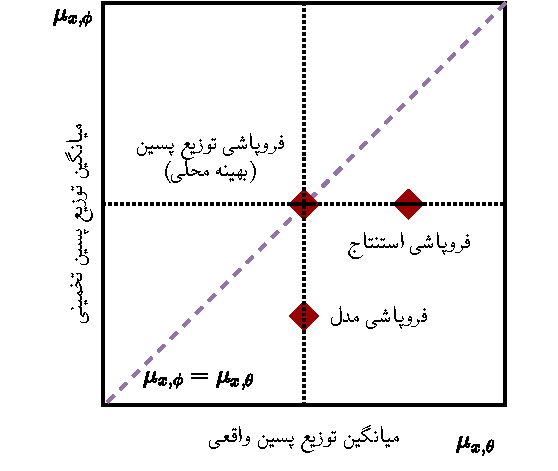
\includegraphics[width=0.5\textwidth]{images/lagging1.pdf}
	\caption{
		نموداری بر فضای میانگین توزیع پسین $(\mu_{x,\phi}, \mu_{x,\theta})$. محور افقی میانگین توزیع \posterior{} مدل و محور عمودی میانگین توزیع \posterior{} تخمینی را نشان می‌دهد. خط چین قطری نیز حالتی را نشان می‌دهد که میانگین توزیع \posterior{} مدل (واقعی) با تخمینی یکسان شده است.
	}
\end{figure}

از آنجا که میانگین \priordist{} برابر صفر است، بنابراین اگر $\mu_{x,\phi} = 0$ شود فروپاشی استنتاج و اگر $\mu_{x,\theta} = 0$ باشد فروپاشی مدل اتفاق افتاده است. لازم به ذکر است که بایستی ابعاد $z$ به گونه‌ای باشد تا بتوان آن را به صورت کارا محاسبه کرد؛ ازین رو $z$ یک عدد یک بعدی در نظر گرفته شده است. محور قطری نیز مربوط به حالتی است که $p_\theta(z|x)$ و $q_\phi(z|x)$ از نظر میانگین با یکدیگر منطبق بوده و توزیع پسین تخمینی، کار خود را به درستی انجام داده است. مبدا نیز مربوط به حالت بهینه محلیِ فروپاشی \posteriordist{} است؛ این در حالی است که احتمالا نقاط بهینه محلی مطلوب‌تر جایی بر روی محور قطری و در اطراف مبدا خواهند داشت.
نمودار‌های زیر حاصل انجام این آزمایش در روند آموزش است.

\begin{figure}[H]
	\centering
	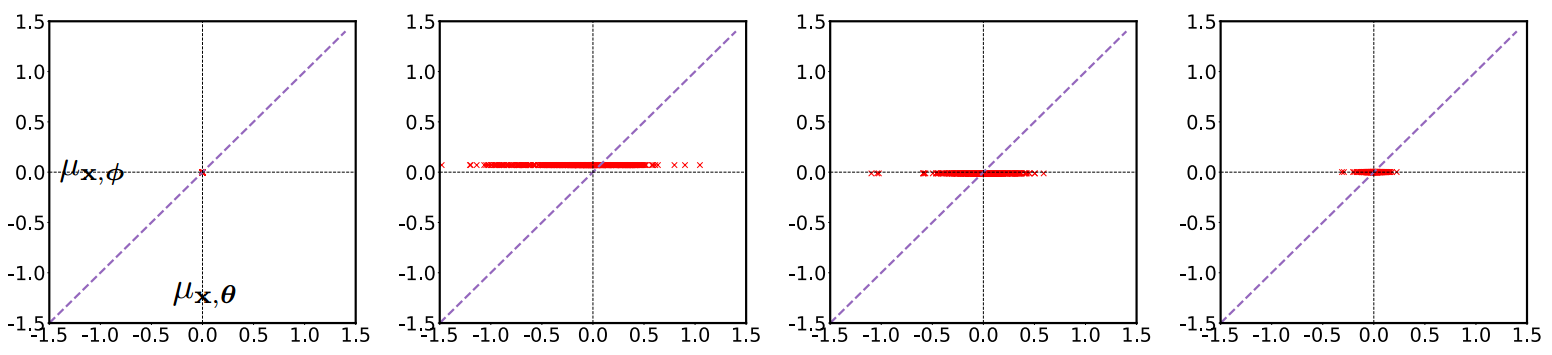
\includegraphics[width=1.\textwidth]{images/lagging2.png}
	\caption{
		نمودارهای فوق از تصویر کردن ۵۰۰ نقطه از داده اصلی بر فضای نهان (در ۴ مقطع زمانی. به ترتیب از شکل سمت چپ به راست، گام آموزشی ۰ ام، ۲۰۰ ام، ۲۰۰۰ ام و انتهایی) بدست آمده است. آنچه که در تصویر فوق مشخص است، آن است که در ابتدای آموزش، دو متغیر $z$ و $x$ از یکدیگر مستقل بوده و در روند آموزش نیز شبکه \encoder{} تخمین صحیحی از \posteriordist{} نداشته و در نتیجه باعث ایجاد حالت فروپاشی استنتاج می‌شود.
	}
\end{figure}
آن طور که از تصاویر برداشت می‌شود به این صورت است که ابتدا نقاط به صورت متمرکز در مبدا جمع شده‌اند  اما در ادامه، نقاط در محور افقی گسترده شده‌اند و در انتها مجددا به سمت متمرکز شدن پیش رفته اند. نکته قابل توجه این است که در تمامی این حالات نقاط در محور افقی پراکنده شده‌اند. برای توجیه این مشاهده می‌توان از صورت دیگری از رابطه \lr{ELBO} بهره برد. می‌دانیم \lr{ELBO} برابر با عبارت زیر است:
\begin{gather}
	\mathcal{L}_{\text{ELBO}}(x;\theta, \phi) = \log p_\theta(x) - {KL}(q_\phi(z|x)~||~ p_\theta(z|x))
\end{gather}
که عبارت اول مربوط به \likelihood{} حاشیه‌ای و عبارت دوم مربوط به فاصله توزیع تخمینی $q_\phi(z|x)$ از توزیع پسین واقعی مدل ($p_\theta(z|x)$) است. واضح است که پارامتر $\phi$ تنها تحت تاثیر عامل \lr{KL} بوده در حالی که پارامتر $\theta$ علاوه بر این، تحت تاثیر عبارت \likelihood{} حاشیه‌ای نیز هست. علاوه بر این تنها عاملی که باعث ایجاد رابطه بین $x$ و $z$ می‌گردد،
\likelihood{}
است و بخش دوم تنها سعی در نزدیک کردن دو توزیع $p_\theta(z|x)$ و $q_\phi(z|x)$ دارد.

حال با نگاه داشتن به رابطه فوق، این پدیده را این طور می‌توان تفسیر نمود که با وجود اینکه ابتدا فضای نهان ساخته شده تقریبا مستقل از فضای داده‌های ورودی است، با پراکنده شدن نقاط به صورت افقی در ادامه روند آموزش، رابطه‌ای بین $z$ و $x$ تحت مدل $p_\theta(x)$ در حال شکل‌گیری است؛ اما به دلیل اینکه شبکه \encoder{} به هیچ عنوان تخمین صحیحی از \posteriordist{} واقعی ندارد و همزمان در حال کمینه کردن هر دو قسمت عبارت \lr{ELBO} نسبت به پارامترهای هر دو شبکه‌ی \encoder{} و \decoder{} هستیم، در نتیجه با ادامه آموزش، رابطه بین این دو متغیر به مرور بر اثر غلبه بخش حاوی فاصله \lr{KL} بر بخش \likelihood{} حاشیه‌ای، از دست رفته و سیستم دچار یک بهینه محلی می‌گردد.


\subsection{راه حل‌های حاشیه‌ای برای رفع مشکل صفر شدن \lr{KL}}
به طور کلی راه حل‌های ارائه شده یا از جنس تغییر معماری ‎\decoder{}‎ و ضعیف کردن قدرت ‎\autoregressive{}‎ آن، تغییر ‎\priordist{}‎ و یا تغییر تابع هزینه هستند.
\\
\begin{figure}[H]
	\centering
	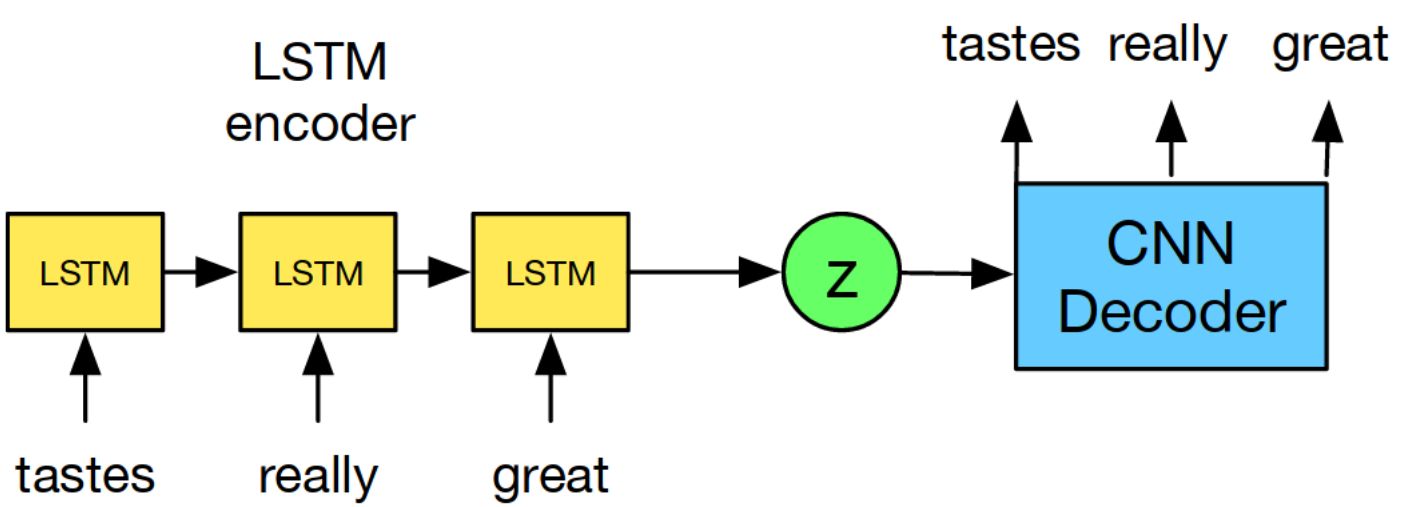
\includegraphics[width=0.5\textwidth]{images/dialated-conv1.png}

	\vspace{0.5cm}

	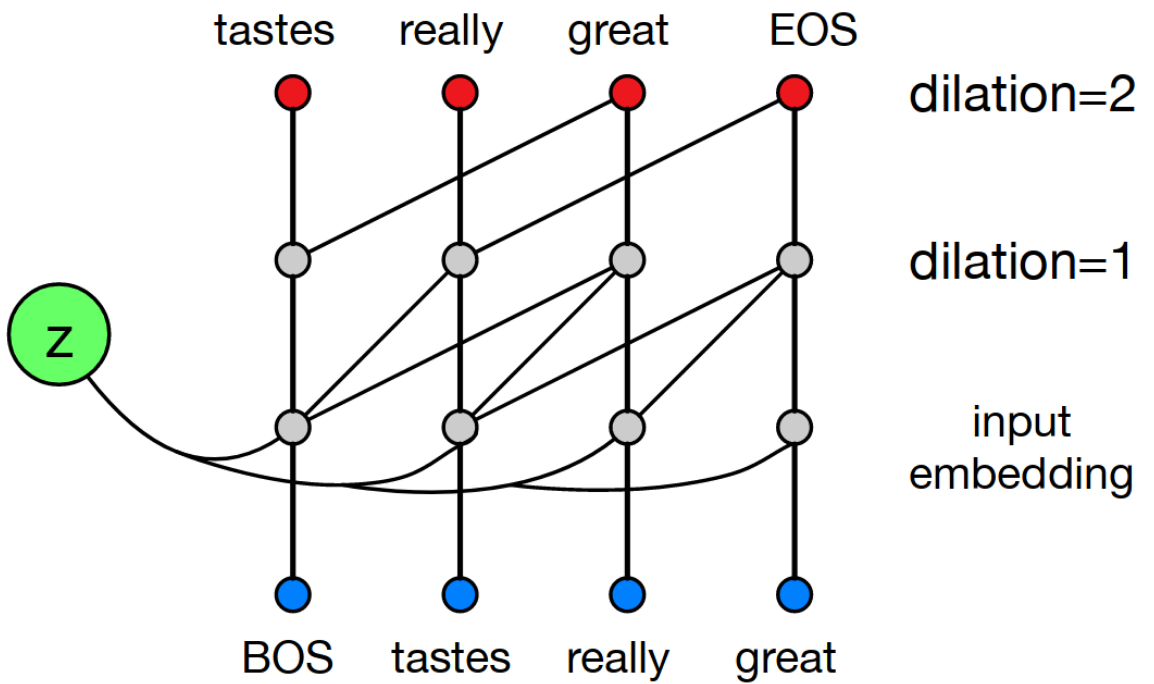
\includegraphics[width=0.5\textwidth]{images/dialated-conv2.png}
	\caption{
		معماری کلی شبکه ارائه شده که از \lr{CNN}  با کانولوشن‌های \dilated{} در  ‎\decoder{}‎ بهره می‌برد.
	}
	\label{fig:dialted_conv}
\end{figure}
راه حل‌های اولیه بیشتر در حوزه تغییر ساختار ‎\decoder{}‎ هستند. دلیل چنین رویکردی در این بود که می‌توان مشکل را در قدرت زیاد مدل‌های ‎\lr{LSTM}‎ در مدلسازی به صورت ‎\autoregressive{}‎ جست و جو کرد؛ چراکه در حوزه تصویر که هر پیکسل مستقل از سایر پیکسل‌ها تولید می‌گردد، چنین پدیده‌ای گزارش نشده است. بنابراین یک راه حل استفاده از مدل‌هایی است که قدرت \autoregressive{} کمتری دارند. برای مثال همان طور که در شکل ‎\ref{fig:dialted_conv}‎ نشان داده شده است، می‌توان ‎\decoder{}‎ را با وام گرفتن از ایده شبکه ‎\lr{PixelCNN}‎ با معماری ‎\lr{CNN}‎ پیاده‌سازی و جایگزین ‎\lr{LSTM}‎ نمود. به طور دقیق‌تر برای پیشبینی هر پیکسل، پیکسل‌های پیش‌رو پوشانده شده، از فیلتر‌های یک بعدی و اتصالات
\trans{\dilated{}}{Dilated}
در کانولوشن‌ها بهره گرفته شده که در نتیجه \trans{\receiptivefield}{Receiptive field}
در هر لایه نسبت به لایه قبل، افزایش نمایی پیدا کند. در واقع با زیاد شدن تعداد لایه‌های با کانولوشن‌های \dilated{}، زمینه طولانی‌تری در خروجی یک گره از لایه مورد نظر دخیل خواهد شد. برای مثال اگر ضریب انبساط ۲ استفاده گردد، \receiptivefield{}‎ در هر لایه نسبت به لایه قبل تقریبا دو برابر شده و در نتیجه از آنجا که میبایست کلمه آخر جمله تابعی از تمام کلمات پیشین باشد،‌ نیاز به $‎\log T$ لایه خواهد بود که $T$ طول بلندترین جمله است. ادعای مقاله بر اساس آزمایش‌های متفاوت بر این است که ساختار ‎\lr{CNN}‎ بیشتر متکی بر فضای نهان  $Z$ بوده و بنابراین مشکل ذکر شده را مقداری تقلیل می‌دهد. نکته قابل ذکر این است که در این حالت نیز اگر ‎اندازه شبکه بسیار بزرگ شود مجددا مشکل صفر شدن ‎\lr{KL}‎ ظهور پیدا می‌کند.

\subsection{\aae} \label{sec:aae}
مدل \trans{\aae}{Adversarial autoencoder}، نسخه تغییر یافته‌ای از مدل \vae{} است تا بخشی از ضعف‌های آن را بپوشاند. همان طور که قبلا نیز توضیح داده شد، تابع هزینه \vae{} از دو بخش تشکیل شده است. بخش اول مربوط به کمینه کردن خطای بازسازی و بخش دوم مربوط به سوق دادن فضای نهان به توزیع گاوسی نرمال است. مدل \aae{}، با حفظ بخش مربوط به خطای بازسازی، در بخش دوم به جای نزدیک کردن توزیع خروجی ‎\encoder{}‎ به  ‎‎\priordist{‎}‎  ($q(z|x) ‎\leftrightarrow p(z)$)، سعی در نزدیک کردن توزیع \trans{\marginal}{Marginal}  خروجی  ‎\encoder{‎}‎  را  به \priordist{} مورد نظر دارد
($q(z) ‎\leftrightarrow  p(z)$).
در واقع توزیع \marginal{} $q(z)$ به صورت زیر تعریف می‌شود:
\begin{gather}
	q(z) = \sum_x p_{data}(x) q(z|x)
\end{gather}
و هدف نزدیک کردن توزیع $q(z)$ به $p(z)$ خواهد بود. بنابراین در مقایسه با مدل \vae{}، اجازه داده می‌شود تا به جای اینکه خروجی \encoder{} به ازای هر نمونه، مستقل از سایر نمونه‌ها به یک توزیع گاوسی نرمال نزدیک شود، توزیع ‎\marginal{}‎ نمونه‌های داده واقعی در فضای نهان، یک توزیع نرمال گاوسی باشد.
\begin{figure}[H]
	\centering
	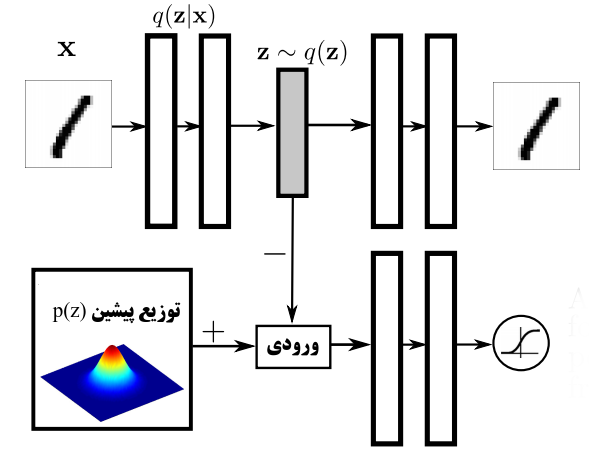
\includegraphics[width=.6\textwidth]{images/aae.png}
	\caption{
		نمایی از مدل  \aae{}. در واقع این مدل، همان مدل \autoencoder{} است که بخش منظم‌ساز مربوط به نزدیک کردن $q(z)$ به $p(z)$ به آن افزوده شده است.
	}
	\label{fig:aae}
\end{figure}
گفته شد که بایستی دو توزیع $p(z)$ و $q(z)$ به یکدیگر نزدیک شوند. حال بر خلاف آنچه که در مدل \vae{} اتفاق می‌افتاد که بخش $KL$ نیاز به محاسبه به صورت فرم بسته داشت، با وام‌گیری از ایده \gan{}، می‌توان \discriminator ‌ای آموزش داد تا نمونه‌های \priordist{} را از نمونه‌های توزیع \marginal
$q(z)$
جدا کند. در واقع اگر بخواهیم با ادبیات شبکه‌های تخاصمی معادل‌سازی کنیم، مولد $q(z)$ و توزیع داده واقعی $p(z)$ خواهد بود که نمایی از این روش نیز در شکل \ref{fig:aae} آمده است. رابطه تابع هزینه این مدل به شکل زیر است:
\begin{gather}
	L_{AAE}(\phi, \theta) = - \expected_{x \sim p_{data}(x), z \sim q_\phi(z|x)} [\log (D(z))] + \expected_{x \sim p_{data}(x), z \sim q_\phi(z|x)}[\log p_\theta(x|z)]\\
	L_{AAE}(D) = - \expected_{z \sim p(z)} [\log D(z)] - \expected_{x \sim p_{data}(x), z \sim q_\phi(z|x)} [\log (1 - D(z))]
\end{gather}
که $q_\phi(z|x)$ توزیع \encoder{}،
$p_\theta(x|z)$
توزیع \decoder{} و $p(z)$ توزیع پیشین است. روند بهینه‌سازی به این صورت است که مانند \gan{} از دو بخش تشکیل شده است؛ بخش بهینه‌سازی خطای بازسازی و بخش تخاصمی. در بخش خطای بازسازی، تنها \autoencoder{} به منظور کاهش خطای بازسازی آموزش داده می‌شود و در بخش تخاصمی، ابتدا \discriminator{} به منظور جداسازی نمونه‌های واقعی از مصنوعی و سپس \encoder{} به منظور نزدیک کردن توزیع \marginal{}‎ فضای نهان به \priordist{} آموزش داده می‌شود.\\
نکته دیگری که می‌توان در نحوه آموزش مدل به آن اشاره نمود این است که کافیست تا بتوانیم از دو توزیع پیشین و حاشیه‌ای \encoder{} نمونه‌برداری کنیم و مانند مدل \vae{}، نیازی به داشتن فرم بسته رابطه بالا نیست که از مزیت‌های این مدل به شمار می‌رود؛ اما از سوی دیگر این مدل بدون پشتوانه نظری و بررسی رابطه آن با \likelihood{} ارائه شد.\\
در مورد نحوه عملکرد ‎\encoder{}‎ چندین گزینه وجود دارد:
\begin{itemize}
	\item \textbf{\deterministic{}:}
	      در اینجا، $q(z|x)$ یک تابع قطعی از $x$ بوده و تنها عامل تصادفی بودن توزیع  $q(z)$، توزیع داده واقعی $p_{data}‎(x)$ است.
	\item \textbf{توزیع \posterior{} گاوسی:}
	      می‌توان خروجی ‎\encoder{}‎ را توزیع گاوسی با ماتریس کوواریانس قطری در نظر گرفت. بنابراین دو عامل تصادفی در $q(z)$ وجود خواهد داشت؛ توزیع داده اصلی و توزیع خروجی ‎\encoder{}‎ . به منظور آموزش مدل مشکلات مشابه آموزش ‎\vae{}‎ وجود دارد که مجددا می‌توان از تکنیک ‎\reparametrization{}‎ بهره برد.
	\item \textbf{\trans{\uniaprox}{Universal approximator} توزیع \posterior{}:}
	      این حالت، کلی‌ترین حالت ممکن برای ‎‎\encoder{}‎ است. ‎\encoder{}‎ به این صورت عمل می‌کند که با گرفتن نویز $‎‎\eta$ (با داشتن توزیع از قبل تعریف شده) و نمونه $x$، یک $z$ در فضای نهان تولید می‌کند. در واقع ‎\encoder{}‎ یک تابع قطعی از $x$ و $‎\eta$ است. مانند حالت قبل، دو عامل تصادفی وجود دارد؛ توزیع داده اصلی و توزیع نویز اولیه. اما بر خلاف مدل قبل، خروجی ‎\encoder{}‎ ، توزیع از پیش تعیین شده‌ای نداشته و با پارامترهای ‎شبکه \encoder{}‎ پارمتریزه می‌شود. در این حالت $q(z)$ به شکل زیر خواهد بود:
	      \begin{gather}
		      q(z) = \sum_x q(z|x) p_{data}(x) = \sum_x \sum_\eta p_{data}(x) p(\eta)  q(z|x, \eta)
	      \end{gather}
\end{itemize}
لازم به ذکر است که در دو حالت اخر، ‎با داشتن دو عامل تصادفی، احتمالا توزیع  ‎\marginal{}‎ ‎\encoder{}‎ ، توزیعی با تغییرات  نَرم‌تر خواهد بود.
\subsection{\wae}
مدل \trans{\wae}{Wasserstein autoencoder} که در ادامه معرفی خواهد شد، نسخه عمومی‌تر مدل \aae{}‎ بوده که به لحاظ تئوری نیز بررسی گردیده است.\\
در بخش ‎\ref{sec:aae}‎ توضیح داده شد که تفاوت ‎\aae{}‎ با مدل ‎\vae{}‎، در نحوه اعمال توزیع مورد نظر بر فضای نهان است. با تکیه بر همین نکته، حالت کلی‌تری از ‎\aae{}‎ به نام ‎\wae{}‎ ارائه شد. در واقع همان طور که در شکل ‎‎\ref{fig:wae}‎ مشخص است، در ‎\vae{}‎ توزیع خروجی ‎\encoder{}‎به ازای هر نمونه به ‎\priordist{}‎ نزدیک می‌شود. در نتیجه این عمل، خروجی ‎\encoder{}‎ به ازای نمونه‌های متفاوت مجبور به داشتن همپوشانی خواهد شد؛ بنابراین بازسازی نمونه‌های داده اصلی از فضای نهان با مشکل مواجه خواهد شد. در مقابل، در ‎\wae{}‎ مقداری دست مدل در نحوه اعمال ‎‎\priordist{}‎ به فضای نهان باز بوده و تنها کافیست توزیع ‎\marginal{}‎ حاکم بر فضای نهان دارای ‎\priordist{}‎ باشد.\\
\begin{figure}[H]
	\centering
	\begin{subfigure}[b]{0.4\textwidth}
		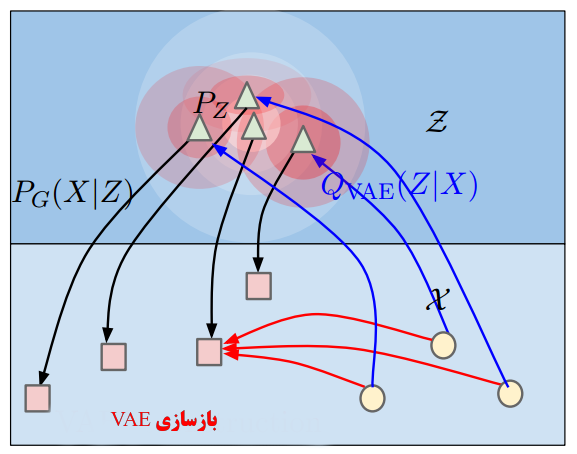
\includegraphics[width=\textwidth]{images/wae1.png}
		\caption{\vae}
		\label{fig:wae-vae}
	\end{subfigure}
	\begin{subfigure}[b]{0.4\textwidth}
		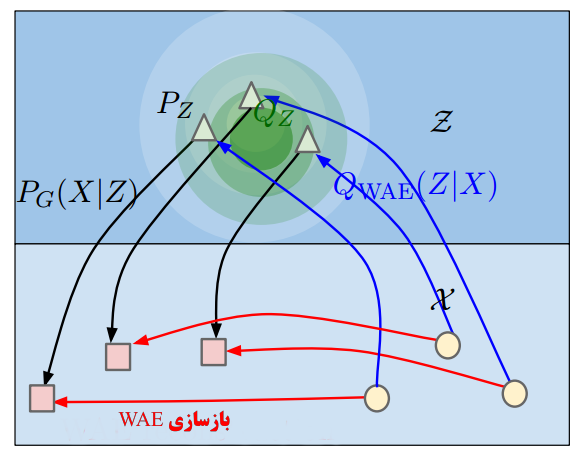
\includegraphics[width=\textwidth]{images/wae2.png}
		\caption{\wae}
		\label{fig:wae-wae}
	\end{subfigure}
	\caption{
		مقایسه نحوه بازسازی در مدل  ‎‎\wae{}‎ با ‎\vae{}‎ . دوایر قرمز رنگ در فضای نهان مربوط به توزیع (گاوسی) خروجی ‎\encoder{}‎ ، دوایر سبز رنگ مربوط به توزیع ‎‎\marginal{}‎ خروجی ‎\encoder{}‎ و  دوایر سفید رنگ، متناظر با ‎\priordist{}‎ (گاوسی نرمال) است. همان طور که در شکل ‎\subref{fig:wae-vae}‎ مشخص است، هر ناحیه قرمز سعی در نزدیک شدن به ناحیه سفید رنگ دارد؛ بنابراین به دلیل وجود همپوشانی بین نواحی مختلف قرمز، مشکلاتی در بازسازی پیش خواهد آمد. این در حالیست که در مدل ‎\wae{}‎ ، تمرکز بر اعمال توزیع گاوسی بر توزیع ‎\marginal{}‎ \encoder{}‎‎ است.
	}
	\label{fig:wae}
\end{figure}
بر خلاف آن که در روش ‎\aae{}‎ اظهار نظری راجع به رابطه تابع هزینه معرفی شده و ‎\likelihood{}‎ مدل ارائه نشد، مدل ‎\wae{}‎ به بررسی این موضوع پرداخته است.
مدل گرافی در نظر گرفته شده برای این روش مانند مدل گرافی ‎\vae{}‎ است. متغیر نهان $z$ ای با توزیعی مشخص و ثابت وجود دارد که نمونه $x$ از آن بدست خواهد آمد. اگر ‎\priordist{}‎ متغیر نهان را با $p_z(z)$ و ‎توزیع ‎‎‎\decoder{}‎‎ را با $p_G(x|z)$ نشان دهیم، توزیع ‎\marginal{}‎
$p_G(x)$
به صورت زیر تعریف می‌شود:
\begin{gather}
	p_G(x) = \sum_z p_z(z) p_G(x|z)
\end{gather}
حال برای اینکه این توزیع را به توزیع $p_{data}‎(x)$ نزدیک کنیم، از فاصله‌های متعددی می‌توان استفاده نمود. در اینجا همان طور که از نام مدل بر‌می‌آید، از فاصله ‎‎\trans{‎\wasser}{Wasserstein}‎‎‎ بهره برده شده است. اگر فاصله ‎‎\wasser{}‎ با تابع هزینه $c$‎ را با $W_c$ نشان دهیم، اثبات شده است که رابطه $W_c(P_{data}‎, P_G)$ را می‌توان به شرح زیر بازنویسی کرد:

\begin{gather}\label{eq:wae_constrained}
	\begin{align}
		W_c(P_{data}, P_G) & = \inf_{\Gamma \in \mathcal{P}(X \sim P_{data}, Y \sim P_G)} \expected_{(X,Y) \sim \Gamma} [c(X,Y)] \nonumber \\
		                   & = \inf_{Q: Q_z = P_z} \expected_{P_{data}} \expected_{Q(Z|X)} [c(X, G(Z))]
	\end{align}
\end{gather}
که $Q_z(z)$، توزیع ‎\marginal{}‎ فضای نهان است؛ به عبارت دیگر:‌$Q_z(Z) = ‎\sum_x q(Z|x)p_{data}‎(x)$

طبق رابطه بالا، به منظور کاهش فاصله ‎\wasser{}‎ بین دو توزیع $P_{Data}‎$ و $P_G$ کافیست توزیع شرطی $Q(Z|X)$ ای بیابیم که توزیع ‎\marginal{}‎ آن برابر با توزیع $P_Z$ باشد. مشکلی که در رابطه ‎\ref{eq:wae_constrained}‎ وجود دارد این است که مسئله بهینه‌سازی با قید است. به منظور رفع این قید می‌توان آن را به شکل زیر بازنویسی کرد:
\begin{gather}
	V_{WAE}(Q, G) = \inf_{G \in \mathcal{G}, ~ Q(Z|X) \in \mathcal{Q}} \expected_{P_{Data}}\expected_{Q(Z|X)} [c(X, G(Z))] + \lambda . D_ Z(Q_Z, P_Z)
\end{gather}
که $‎\mathcal{Q}‎$  و ‎$‎\mathcal{G}$ خانواده توابعی هستند که با شبکه عصبی توانایی مدل کردن آن‌ها را داشته و $D_Z(. , .)$ هم می‌تواند هر فاصله‌ای بین دو توزیع $Q_Z$ و $P_Z$ باشد (تنها کافیست بتوان از آن نسبت به پارامترهای شبکه مشتق گرفت). لازم به ذکر است که در رابطه بالا، لزومی به تصادفی بودن خروجی ‎\encoder{}‎ نبوده و حالت  ‎\deterministic{}‎ هم می‌تواند داشته باشد.\\
حال اینکه به جای $D_Z(. , .)$ از چه معیار یا روشی استفاده گردد، در این مقاله دو گزینه ارائه شده است که بیان خواهند شد:
\begin{itemize}
	\item \textbf{مبتنی بر معماری تخاصمی:}
	      میدانیم ‎\gan{}‎‌ها فاصله ‎\lr{JS}‎ را کمینه می‌کنند. به منظور کمینه کردن $D_Z(. , .)$ نیز می‌توان از این فاصله بهره برد. به این صورت که یک شبکه ‎\discriminator{}‎ برای تمیز دادن نمونه‌های ‎\priordist{}‎ از ‎‎نمونه‌های حاصل از خروجی ‎\encoder{}‎ استفاده می‌گردد؛ از سوی دیگر ‎\encoder{}‎ سعی در تولید نمونه‌هایی خواهد داشت که به نمونه‌های ‎\priordist{}‎ نزدیک بوده و ‎\discriminator{}‎ به اشتباه بیفتد. بنابراین اگر تمیزدهنده را با $D$ نشان دهیم، توابع هزینه به شکل زیر خواهد بود:
	      \begin{gather}
		      V(Q, G)= \inf_{Q, G} \expected_{P_{Data}}\expected_{Q(Z|X)} [c(X, G(Z))] - \lambda (\expected_{P_{Data}}\expected_{Q(Z|X)} [\log D(Z)]) \nonumber \\
		      V(D)= \sup_{D} \expected_{P_{Data}}\expected_{Q(Z|X)} [\log (1-D(z))] + \expected_{P(Z)} [\log D(Z)]
	      \end{gather}
	\item \textbf{مبتنی بر فاصله \mmd :}
	      برای تابع کرنل مثبت معین \trans{‎\reproducing}{Reproducing} ؟؟؟
	      $k: ‎\mathcal{Z} ‎‎\times \mathcal{Z} ‎\rightarrow ‎\mathbb{R}‎‎$
	      رابطه ‎\mmd{} ‎ یا ‎\lr{Maximum Mean Disrepancy} به شکل زیر تعریف می‌شود:
	      \begin{gather}
		      \mathsf{MMD}_k(P_Z, Q_Z) = {\vert \vert \int_\mathcal{Z} k(z, .) dP_Z(z) - \int_\mathcal{Z} k(z, .) dQ_Z(z) \vert \vert}_{\mathcal{H}_K}
	      \end{gather}
	      به طوری که $‎\mathcal{H}‎_K$، یک  ‎\lr{RKHS (Reproducing ‎ Kernel ‎ Hilbert ‎ Space)}‎ برای توابع از $‎\mathcal{Z}‎$ به اعداد حقیقی است. اگر تابع $k$ ویژگی‌های مشخصی را داشته باشد، ‎\mmd{}‎ را به یک متر تبدیل کرده و این امکان را فراهم می‌کند تا از این متر به عنوان تابع هزینه برای کمینه کردن فاصله $P_Z$  و $Q_Z$  بهره برده شود. از آنجا که رابطه بالا به طور مستقیم قابل محاسبه و بهینه‌سازی نیست، از تخمین‌گر نااریب زیر استفاده می‌گردد. اگر $n$ نمونه از دو توزیع $P_Z$ و $Q_Z$ داشته و به ترتیب با $z_i$ و $‎\tilde{z}_i$ نشان داده شوند،‌خواهیم داشت:
	      \begin{gather}
		      \begin{align*}
			      \mathsf{MMD}_k(z_{1,2,...,n};\tilde{z}_{1,2,...,n}) = & \frac{1}{n(n-1)} \sum_{l \neq j} k(z_l, z_j) +
			      \frac{1}{n(n-1)} \sum_{l \neq j} k(\tilde{z}_l, \tilde{z}_j)                                              \\
			                                                            & - \frac{1}{n ^ 2} \sum_{l, j} k(z_l, \tilde{z}_j)
		      \end{align*}
	      \end{gather}
\end{itemize}‎
بدست آمدن نمونه از توزیع $P_Z$ واضح است و برای نمونه‌برداری از توزیع $Q_Z$ نیز با استفاده از روش
\trans{\ancestral{}}{Ancestral}
‎ ابتدا از توزیع $P_{data}‎$ نمونه‌برداری کرده و سپس از توزیع $Q(Z|X)$ نمونه‌برداری انجام می‌گیرد.
نکته قابل ذکر این است که قضایا ارائه شده تنها در حالتی که ‎\decoder{}‎ تابعی قطعی باشد صادق هستند؛ البته قضیه مشابهی نیز تنها برای تابع هزینه مجذور فاصله ارائه شده است.
\subsection{دیگر روش‌های جلوگیری از صفر شدن فاصله \lr{KL}}
آنچه که تا به حال توضیح داده شد، روش‌هایی بودند که به نظر موثرتر و پایه‌ای تر به موضوع پرداخته بودند؛ اما مقالات بسیاری در این حوزه ارائه شده است که در ادامه به توضیح خلاصه‌ای از آن‌ها خواهیم پرداخت.

نوع دیگری از مدل‌های مولد موجود است که تا به حال چندان نه در حوزه تصویر و به مراتب بیشتر در حوزه متن مورد توجه قرار نگرفته اند. در ادامه به توضیح این دسته نیز پرداخته خواهد شد.
\subsection{\normalizingflownets{}}
در کنار دو عضو بزرگ از خانواده شبکه‌های مولد مبتنی بر \vae{} و \gan{}، نوع دیگری از شبکه‌ها به نام \normalizingflownets{} وجود دارند. یکی از مشکلات اساسی ما در این دو نوع \vae{} و \gan{} این است که توانایی محاسبه \likelihood{} به صورت کارا و بدون استفاده از کران‌های پایین و یا بالا وجود ندارد. برای مثال در \vae{} کران پایین \likelihood{} را بیشینه کرده و در \gan{}‌ها نیز از تابع هزینه دیگری استفاده می‌شود و در مورد رابطه آن با \likelihood{} صحبت شفافی نمی‌توان کرد (عدم امکان محاسبه \likelihood{} در \gan{} به صورت کلی بیان شد؛ این در حالی است که در حوزه متن امکان محاسبه آن وجود دارد).  بر خلاف این دو دسته، خانواده \normalizingflownets{} توانایی نمونه‌گیری و محاسبه \likelihood{} به صورت کارا را داشته و یا حداقل سعی بر این موضوع دارند. بنابراین امکان بهینه‌سازی مدل نسبت به تابع هزینه‌ای بر مبنای مقدار دقیق \likelihood{} امکان پذیر است. از سوی دیگر همان طور که تا به اینجا توضیح داده شد، سختی‌ها و نقاط ضعفی از قبیل تنوع نداشتن نمونه‌ها در \gan{} و یا صفر شدن بخش \lr{KL} در \vae{} وجود دارد. این در حالیست که در \normalizingflownets{} با بهینه‌سازی بر اساس \likelihood{} مشکل کم بودن تنوع نمونه‌ها وجود نداشته و یا مشکلات آموزش مانند آنچه ذکر شد، گزارش نشده است. البته این نکته قابل ذکر است که در صورت کم بودن ظرفیت مدل نسبت به توزیع هدف مورد نظر، تابع هزینه مبتنی بر \likelihood{} رفتار میانگین جویانه از خود بروز داده و توزیعی را یاد خواهد گرفت که تمام نقاط را پوشش دهد. بدیهیست که ممکن است برای پوشش دادن تمام نقاط نقاطی نامطلوب را نیز پوشش دهد.
\subsubsection{مفاهیم پایه}
فرض کنید 
${\bf{ Z}} \in \mathbb{R}^{D}$
متغیر تصادفی با تابع چگالی احتمال مشخص
$p_{\bf Z}: \mathbb{R}^D$
 و $\bf f$ تابعی معکوس پذیر و 
 ${\bf Y} = {\bf f}({\bf Z})$
 است. حال با استفاده از قانون تغییر متغیر می‌توان رابطه زیر را نوشت:
 \begin{align}  \label{eq:flow_target_dist} 
   p_{\bf Y}({\bf y}) =& p_{\bf Z}({\bf g}({\bf y})) 
   |\text{det} ~ \text{D} {\bf g}({\bf y})|
   \nonumber \\
   =& p_{\bf Z}({\bf g}({\bf y})) 
   |\text{det} ~ \text{D} {\bf f}({\bf g}({\bf y}))|^{-1}
 \end{align}
که $\bf g$ تابع معکوس $\bf f$ و 
$\text{D} {\bf g}({\bf y}) = \frac{\partial {\bf g}}{\partial {\bf y}}$
ماتریس ژاکوبین تابع $\bf g$ و 
$\text{D} {\bf f}({\bf z}) = \frac{\partial {\bf f}}{\partial {\bf z}}$
ماتریس ژاکوبین تابع $\bf f$ است. تابع چگالی احتمال حاصل از اعمال تابع $\bf f$ به توزیع پایه را با 
$f_*p_{\bf Z}$
نشان خواهیم داد.

در ادبیات مدل‌های مولد، تابع $\bf f$ به عنوان مولد، توزیع پایه 
$p_{\bf z}$ 
را به توزیعی پیچیده‌تر تبدیل می‌کند که به حرکت از توزیع پایه به توزیع نهایی را جهت مولد می‌نامند. به منظور نمونه‌برداری از توزیع نهایی نیز می‌توان از توزیع پایه نمونه برداری کرده و با استفاده از تابع 
${\bf y} = {\bf f} ( {\bf z} )$
به نمونه از توزیع نهایی رسید. در جهت مخالف، برای تبدیل توزیع نهایی به توزیع پایه که معمولا توزیع گاوسی نرمال انتخاب می‌شود، از تابع $\bf g$ بهره برده می‌شود. به همین دلیل انتخاب نام جریان نرمال‌کننده بدون هدف نبوده و در واقع جهت مخالف مربوط به تبدیل توزیع پیچیده نهایی به توزیع پایه گاوسی نرمال است. 
\\
به طور کلی اگر تابع $\bf f$ یک تبدیل پیچیده باشد، توانایی تولید هر توزیعی وجود خواهد داشت؛ به عبارت دیگر به ازای هر توزیع هدف 
$ p_{\bf Y}({\bf y})$
تابع $\bf f$ای وجود خواهد داشت که 
$ p_{\bf Y}({\bf y}) = f_*p_{\bf Z}$.
اما به منظور آموزش و نمونه‌گیری کارا، نیاز است تا این توابع ویژگی‌های خاصی به شرح ذیل داشته باشند:
\begin{itemize}
    \item 
معکوس‌پذیر باشند. ممکن است تابع معکوس در جهت نمونه‌گیری و یا جهت نرمال‌ساز به کار برده شود.
    \item 
    به اندازه کافی پیچیده باشند تا بتواند توزیع داده اصلی را مدل کنند.
    \item 
    به لحاظ محاسباتی کارا باشند. برای محاسبه \likelihood{} یک نمونه و نمونه‌گیری نیاز است تا هر دو جهت نمونه‌گیری و نرمال‌ساز به صورت کارا محاسبه شوند. علاوه بر این، طبق رابطه \ref{eq:flow_target_dist} برای محاسبه  \likelihood{} یک نمونه در توزیع نهایی، به محاسبه کارای دترمینان ماتریس ژاکوبین تابع $\bf f$ نیاز است. بنابراین بایستی دترمینان ماتریس ژاکوبین تابع $\bf f$ نیز به صورت کارا محاسبه شود.
\end{itemize}
لایه لایه فلو دار
این خانواده از مدل‌های مولد شامل چندین دسته هستند که در ادامه معرفی خواهند شد.
\subsubsection{جریان‌های 
\trans{\elementwise{}}{Elementwise}}
\subsubsection{جریان‌های خطی}
\subsubsection{جریان‌های اتصالی}
\subsubsection{جریان‌های \autoregressive{}}


\section{\condtg}
در ادامه ابتدا به دلیل مشابهت مدل‌های مولد شرطی و غیر شرطی، به معرفی تعدادی از معروف‌ترین مدل‌های مولد غیر شرطی پرداخته، سپس چند مورد مدل مولد شرطی ساده و در نهایت یکی از کامل‌ترین مدل‌های مولد شرطی موجود معرفی و در بخش آخر نیز پس از ارائه روش پیشنهادی، کارهای آتی بیان خواهد شد.
از آنجا که تولید متن به صورت شرطی شباهت زیادی به عملیات تولید متن و دنباله‌های گسسته دارد، در این بخش به شرح این دسته از مدل‌ها پرداخته خواهد شد.

مدل بعدی، مدل‌های \trans{خودرمزنگار وردشی}{Variational autoencoder} هستند \cite{vae-org}. با معرفی این دسته از مدل‌ها، موج جدیدی در حوزه مدل‌های مولد به طور خاص مدل‌های مولد تصویر ایجاد شد اما بر خلاف آن، عملکرد چندان مناسبی در حوزه متن کسب نکردند \cite{vae-text} که پس از معرفی مدل به دلایل عملکرد ناموفق آن اشاره خواهد شد.\\
\subsection{مدل‌های شرطی ساده}
ساده‌ترین رویکردی که در مدل‌های شرطی مورد استفاده قرار می‌گیرد، دخیل کردن شروط مورد نظر به ورودی مولد است. در روش جبر معلم می‌توان شرط را به بردار \trans{تعبیه}{Embedding} و  یا در صورت داشتن بردار نهان، به انتهای بردار نهان ابتدایی مدل مولد متصل نموده و تحویل مدل مولد داد. در واقع مدل مولد به تنهایی بایستی هم ساختار جمله و هم اعمال شروط مورد نظر را به جمله یاد بگیرد. در مورد شبکه‌های \vae{} این شروط، هم به کدگذار و هم به کدگشا داده خواهد شد \cite{cvae} و در مورد\gan{} نیز به مولد و تمیزدهنده ورودی داده خواهد شد \cite{cgan}. از آنجا که این مدل‌ها روش‌هایی ساده و در مورد شبکه‌های \vae{} و مقابله‌ای تقریبا آزمایش شده تنها در حوزه تصویر هستند، به تنهایی چندان کاربرد وسیعی در حوزه متن ندارند و به عنوان مدل پایه از آن‌ها بهره برده ‌می‌شود. نسخه دیگری از \gan{} نیز وجود دارد که به منظور تولید جمله با $k$ قطبیت معین، به ازای هر مقدار شرط یک مدل مولد مجزا و یک \trans{دسته‌بند}{Classifier} بین $k+1$ دسته آموزش می‌دهد \cite{sentigan}؛ در این دسته‌بند یک دسته نشانگر داده مصنوعی و سایر دسته‌ها نشان‌گر مقادیر شرط هستند. به عبارت دیگر در مجموع $k+1$ شبکه آموزش داده خواهد شد. مشخص است که با افزایش تعداد شرط‌ها، این مدل مقیاس‌پذیر نخواهد بود.
\subsection{\towardctg}
شاید این روش یکی از کامل‌ترین روش‌های ارائه شده برای تولید جملات شرطی باشد. بر خلاف مدل‌های ساده قبلی که رابطه بین شروط را در نظر نمی‌گرفتند، این روش علاوه بر تولید جملات صحیح و مرتبط با حالت شرط مورد نظر، سعی در حفظ ساختار و معنای کلی جمله با داشتن حالات مختلف شرط دارد \cite{toward}.
\begin{figure}[h]
	\centering
	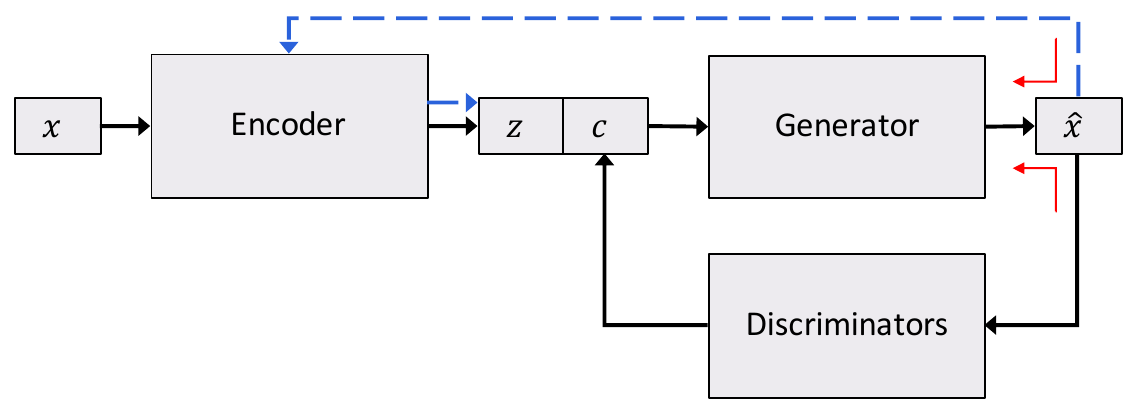
\includegraphics[width=0.5\textwidth]{images/toward1.png}
	\caption{
		نمایی نحوه آموزش مدل \towardctg. خط‌های آبی و سفید جهت حرکت داده و خط‌های قرمز جهت انتفال گرادیان را مشخص می‌کنند.
		\cite{toward}.}
	\label{fig:toward}
\end{figure}
همان‌طور که در شکل \ref{fig:toward} مشخص است، این مدل از ۳ بخش کلی تشکیل شده است؛ یک کدگذار، یک مولد و یک یا چند تمیزدهنده که در شکل به جهت سادگی تنها یک نمونه از آن آورده شده است. اگر $c$ نشانگر شرط مورد نظر باشد، وظیفه کدگذار کد کردن جمله ورودی به فضای نهانی است که $c$ در آن ظاهر نشده باشد؛ از سوی دیگر مولد یا در ادبیات مدل‌های پیشین همان کدگشا وظیفه برگرداندن متغیر نهان بدست آمده از کدگذار به جمله اصلی البته با در نظر گرفتن شرط $c$ را داشته و در نهایت تمیزدهنده موظف به نظارت بر وجود و رعایت شرط $c$ در جمله تولید شده توسط مولد است. در واقع می‌توان مدل را به صورت یک \vae{} شرطی به همراه یک شبکه تمیزدهنده دید که وظیفه نظارت بر شرط مورد نظر را دارد. جهت آموزش این مدل و در نظر گرفتن ویژگی‌های ذکر شده، تابع هزینه از چندین قسمت تشکیل شده است که به اختصار راجع به آن‌ها توضیح داده خواهد شد.\\

\subsubsection*{آموزش کدگذار و مولد}
مطابق با آنچه توضیح داده شد اولین بخش از تابع هزینه مربوط به تابع هزینه شبکه‌های \vae{} شرطی ساده بوده که کنترل‌کننده وظیفه کد کردن و برگرداندن آن به جمله با ویژگی مورد نظر را بر عهده دارد. اگر $E$ کدگذار، $G$ مولد و $D$ تمیزدهنده باشد، خواهیم داشت:
\begin{equation}
	\begin{split}
		L_{VAE} (E, G) =& \expected_{x \sim p_{data}(x)} [KL (q_E(z|x) || N(\textbf{\latin{0}},\textbf{\latin{I}})) - \expected_{q_E(z|x)q_D(c|x)} [\log p_G(x|z,c)]].
	\end{split}
\end{equation}
از سوی دیگر باید جمله تولیدی توسط مولد حامل ویژگی مورد نظر باشد. بنابراین تابع هزینه ذیل در نظر گرفته شده است:
\begin{equation}
	\begin{split}
		L_{att, c} (G) =& -\expected_{z \sim p(z), c \sim p(c)} [\log q_D(c|G(z, c))]]
	\end{split}
\end{equation}
که $p(c)$ و $p(z)$
\trans{توزیع پیشین}{Prior distribution}
تعریف شده روی متغیرهای مربوطه هستند. به عبارت دیگر ابتدا تعدادی نمونه $z$ و $c$ با استفاده از توزیع‌های پیشین تعریف شده ایجاد نموده و سپس مولد بایستی جملاتی را تولید نماید که درست‌نمایی شروط در تمیزدهنده‌های مربوطه بیشینه شود.\\
آخرین تابع هزینه‌ای که برای این بخش از مدل در نظر گرفته شده مربوط به حذف وابستگی بین متغیرهای $z$ و $c$ است. به عبارت دیگر مولد بایستی $z$ و $c$ را به جمله‌ای تبدیل نماید که اگر این جمله توسط کدگذار مجددا کد گردد، همان $z$ اولیه بدست آید و جنبه دیگری غیر شروط مورد نظر در جمله تغییر نکرده باشد. این تابع به شکل زیر تعریف گردیده است:
\begin{equation}
	\begin{split}
		L_{att, z} (G) =& -\expected_{z \sim p(z), c \sim p(c)} [\log q_E(z|G(z, c))]].
	\end{split}
\end{equation}
در واقع از سوی دیگر می‌توان کدگذار را به عنوان یک تمیزدهنده‌ مشاهده کرد که وظیفه نظارت بر حفظ محتوای جمله غیر از شروط مورد نظر را دارد.
\subsubsection*{آموزش تمیزدهنده}
بخش دیگر مربوط به آموزش تمیزدهنده می‌باشد؛ اینکه تمیزدهنده برچسب شرط هر جمله را به درستی پیش‌بینی کند. لازم به ذکر است که برای هر ویژگی یا شرط، یک تمیزدهنده مستقل وجود دارد. برای مثال اگر یک ویژگی زمان فعل و دیگری قطبیت آن باشد، دو تمیزدهنده، یکی برای زمان فعل و دیگری برای قطبیت آموزش داده خواهد شد. بخش اول تابع هزینه شبکه تمیزدهنده به شکل ذیل است:

\begin{equation}
	\begin{split}
		L_{s} (D) =& -\expected_{(x,c) \sim p_{data}(x,c)} [\log q_D(c|x)].
	\end{split}
\end{equation}
از آن‌جایی که برچسب‌های تمیزدهنده در روند آموزش مورد استفاده قرار می‌گیرد بنابراین برچسب‌زنی‌های با قطعیت پایین می‌تواند منجر به عدم پایداری آموزش گردد. به این منظور تابع هزینه زیر نیز در نظر گرفته می‌شود.
\begin{equation}
	\begin{split}
		L_{u} (D) =& -\expected_{z \sim p(z), c \sim p(c), x \sim p_G(x|z,c)} [\log q_D(c|x) + \beta H(q_D(c'|x))]
	\end{split}
\end{equation}
که $H(q)$ آنتروپی توزیع $q$ و $\beta$ ضریب تنظیم کننده است.
در نهایت توابع هزینه به شکل زیر خواهند بود:
\begin{equation}
	\begin{split}
		L (D) &= L_{s} (D) + \lambda_u L_{u} (D)\\
		L (G) &= L_{VAE} (G) + \lambda_c L_{att, c} (G) + \lambda_z L_{att, z} (G)\\
		L (E) &= L_{VAE} (E)
	\end{split}
\end{equation}
که $(\lambda_s, \lambda_u, \lambda_c , \lambda_z)$ همگی ضرایب تنظیم‌کننده هستند. از دیگر نقاط قوت این مدل باید به دو مورد زیر نیز اشاره نمود:
\renewcommand{\labelitemi}{$\bullet$}
\begin{itemize}
	\item

	      آموزش\trans{نیمه‌نظارتی}{Semi-supervised}:
	      همان‌طور که در روابط و نمای کلی مدل مشخص است، تابع هزینه $L_{VAE}$ نیازی به داده برچسب زده شده نداشته و به شکل  \trans{\unsupervised}{Unsupervised} آموزش می‌بیند. در واقع برای آموزش کل مدل به تعداد زیادی جمله بدون برچسب و تعداد کمتری که در حدود ۳۰۰ جمله که در مقاله ادعا شده است برای برچسب‌زنی نیاز است.
	\item
	      عدم نیاز به داده \trans{جفت برچسب زده شده}{Jointly labeled}:
	      از آنجا که هر شرط مستقل از سایر شروط و برای هر یک، یک تمیزدهنده و آموزش مجزا در نظر گرفته شده است، بنابراین نیازی به داده جفت برچسب‌زده شده نیست.
\end{itemize}